\documentclass[letterpaper,10pt,conference]{ieeeconf}

\providecommand{\IEEEoverridecommandlockouts}{}
\providecommand{\overrideIEEEmargins}{}
\IEEEoverridecommandlockouts
\overrideIEEEmargins

\usepackage{amsmath,amssymb,amsfonts}
\usepackage{bm}
\usepackage{booktabs}
\usepackage{multirow}
\usepackage{graphicx}
\usepackage{cite}
\usepackage{url}
\usepackage{xcolor}
\usepackage{enumitem}

\DeclareMathOperator{\Log}{Log}
\DeclareMathOperator{\Exp}{Exp}

\title{\LARGE \bf
Task Frames Are Too Coarse:
Learning Phase-Dependent Generator Relevance for Geometric Skill Transfer
}

\author{Anonymous Authors}

\begin{document}
\maketitle

\begin{abstract}
Learning from demonstration must adapt skills when task objects move, but
task-parameterized methods often treat each reference frame as a single
relevance unit. We argue that this unit is too coarse because the translation
and rotation generators inside one relation can obey different task constraints
across skill phases. We introduce a phase-dependent generator relevance
representation that selects which relation changes should propagate and lets
rigid-body geometry realize the selected finite motion. The learned
transformation law is inspected with isolated generator interventions, while
symmetric execution is evaluated with quotient task-space metrics. In a
keyed-to-circular insertion task, the method recovers a sharp phase switch:
lateral translation remains relevant, axial yaw is propagated while the key
constrains the gate, and the same yaw generator is suppressed after physical
clearance. A matched circular-placebo intervention further contains a visible
yaw sweep without any axial-yaw intervention response, separating trajectory
statistics from task relevance. Fixed-context replications, few-shot tests,
rotation-of-the-world controls, and circular symmetry interventions support
assigning geometric task relevance to generators rather than frames.
\end{abstract}

\section{Introduction}
\label{sec:intro}

Learning from demonstration is attractive for robot manipulation because it
allows a robot to reuse a small set of successful examples instead of requiring
a manually programmed controller for every new scene
\cite{Argall2009Survey,Ravichandar2020Recent}. A central difficulty,
however, is geometric generalization: the objects and relations that define a
task change between demonstration and execution. Task-parameterized movement
models address this problem by expressing demonstrations in object- or
relation-centered frames and adapting the learned motion to new frame
configurations \cite{Calinon2016Tutorial,Calinon2014TPGMM,Calinon2018TPModels}.
This perspective has supported a broad family of probabilistic and
task-parameterized skill representations, including methods that learn task
priorities, select or weight reference frames, or reduce the number of
demonstrations required for transfer
\cite{Huang2018GeneralizedTP,Silverio2019TaskPriorities,Sena2019FrameWeighted,
Zhu2022FewTP,Sun2024FrameWeighted,Montero2024TPGP}.

The reference frame itself nevertheless remains a coarse unit of geometric
relevance. A frame bundles several translation and rotation generators into one
object, although these generators need not share the same task meaning. Consider
a task relation $C_r\in SE(3)$ between an insertion target and the world. If the
target is translated laterally, the demonstrated trajectory should generally
translate with it. If a non-axisymmetric keyed peg is rotated about the
insertion axis, its orientation must also follow that rotation. For a circular
peg, in contrast, the same axial rotation is a continuous symmetry of the task:
the target relation has changed as a rigid frame, yet the physical insertion
requirement has not. A single scalar frame weight therefore faces an intrinsic
conflict. Suppressing the frame to ignore the irrelevant yaw also suppresses the
still-relevant translations; following the frame to preserve translations
incorrectly propagates yaw.

This issue is distinct from whether a model can produce anisotropic outputs.
Task-parameterized Gaussian models can induce directional behavior through
their local covariance structure \cite{Calinon2014TPGMM,Calinon2018TPModels},
and recent multi-reference-frame Gaussian-process models learn a
time-dependent relevance for each reference frame \cite{Montero2024TPGP}.
Similarly, modern equivariant robot policies exploit known group structure to
improve sample efficiency and generalization
\cite{Cohen2016GECNN,Simeonov2022NDF,Ryu2024DiffusionEDF,Yang2024EquiBot,
Gao2024RiEMann}. These approaches motivate a sharper representation question:
\emph{is the frame the right atomic unit of task relevance?} We instead ask
which individual generators of a task relation should be propagated to the
skill, and when. The answer need not be full equivariance or full invariance,
and need not be shared by all generators of the same frame.

We formulate this question through a phase-dependent generator relevance
operator. A task-relation perturbation is first represented in a physically
meaningful Lie-algebra basis. The operator
$\mathbf P_r(s)$ then selects the amount of each generator that should be
transferred at skill progress $s$. The selected finite transformation is applied
through the task relation itself rather than approximated by an unconstrained
trajectory Jacobian. This separates \emph{what geometric change is relevant}
from \emph{how that finite change acts on the demonstrated trajectory}.

A second consequence is that evaluation must distinguish task equivalence from
robot-space realization. For an axisymmetric insertion, poses that differ only
by axial spin lie in the same task-equivalence class. Penalizing this spin in an
ordinary pose metric measures a motion-planner or inverse-kinematics choice,
not task error. We therefore evaluate three levels separately: generator-law
recovery, quotient task-space error, and raw realization error.

The paper makes four contributions:
\begin{itemize}[leftmargin=*,itemsep=1pt,topsep=2pt]
    \item We move the unit of task relevance from the frame to the generator by
    introducing a phase-dependent relevance operator
    $\mathbf P_r(s)$ that explicitly models heterogeneous relevance among
    generators of the same task relation, with scalar frame weighting, full
    equivariance, and invariance as nested special cases.
    \item We separate generator relevance from finite geometric realization and
    state an excitation condition that distinguishes an \emph{unidentified}
    generator from a genuinely invariant one.
    \item We propose a symmetry-aware evaluation protocol combining
    isolated-generator response recovery with quotient task-space distance for
    tasks possessing a continuous symmetry subgroup.
    \item We construct a controlled keyed-to-circular insertion benchmark in
    physics simulation and compare against full equivariance, scalar
    frame weighting, rotation-aware TP-GMM, generic conditional regressors, and
    dense operator ablations. The results show that frame-level relevance is
    structurally too coarse when translation and axial rotation of the same
    relation have different phase-dependent relevance.
\end{itemize}

\section{Related Work}
\label{sec:related}

\subsection{Task-Parameterized Skill Learning}

Task-parameterized models encode a skill relative to frames that describe the
current situation. TP-GMM and related models transform local Gaussian
statistics into the current task frames and combine them through Gaussian
products, allowing both Gaussian means and covariances to vary with the task
parameters \cite{Calinon2014TPGMM,Calinon2016Tutorial,Calinon2018TPModels}.
Extensions have addressed task priorities, redundant frames, and limited
demonstration data \cite{Huang2018GeneralizedTP,Silverio2019TaskPriorities,
Zhu2022FewTP}. These models are important baselines here because their
covariance structure can create implicit anisotropic responses; our claim is
not that TP-GMM is isotropic, but that the transformation law associated with
individual relation generators is not an explicit learned object.

\subsection{Reference-Frame Relevance}

Frame-weighted trajectory generation improves extrapolation by estimating the
importance of task parameters rather than treating all frames equally
\cite{Sena2019FrameWeighted}. Sun \emph{et al.} further learn reference-frame
weights along task progress to support learning from few demonstrations
\cite{Sun2024FrameWeighted}. Montero \emph{et al.} learn a local GP in each
reference frame and a second self-supervised GP that predicts frame relevance
at every time step \cite{Montero2024TPGP}. These methods motivate our comparison
to phase-dependent frame relevance. The key distinction is granularity:
a scalar weight $w_r(s)$ acts on the frame as a whole, whereas our operator
allows different generators of the same relation to have different relevance.

\subsection{Equivariance and Geometric Robot Learning}

Equivariant representations have recently improved the data efficiency and
geometric generalization of visuomotor learning. Neural Descriptor Fields
encode SE(3)-equivariant object descriptors \cite{Simeonov2022NDF};
Diffusion-EDFs imposes bi-equivariance on SE(3) diffusion
\cite{Ryu2024DiffusionEDF}; EquiBot introduces a SIM(3)-equivariant diffusion
policy \cite{Yang2024EquiBot}; and RiEMann directly learns SE(3)-equivariant
manipulation policies \cite{Gao2024RiEMann}. Such approaches exploit known
symmetry groups. In contrast, we study \emph{task-dependent symmetry
selection}: the same geometric generator can be relevant in one task and
irrelevant in another, and its relevance can vary with task progress.

\section{Method}
\label{sec:method}

\textbf{Overview.}
The method follows a structured geometric transfer chain:
\[
C_r^0\!\rightarrow C_r
\Rightarrow \bm c_r
\Rightarrow \mathbf P_r(s)\bm c_r
\Rightarrow C_r^{\rm sel}(s)
\Rightarrow \hat X(s).
\]
Only the phase-dependent operator $\mathbf P_r(s)$ is learned. The remaining
steps are fixed by the selected task-relation coordinates, the nominal
trajectory, and the finite action of $SE(3)$. This separates \emph{which}
relation generators are task-relevant from \emph{how} a selected finite relation
change moves the demonstrated trajectory.

\subsection{Problem Formulation and Task-Relation Coordinates}
\label{sec:problem_formulation}

Let $C_r^0,C_r\in SE(3)$ denote the nominal and current configurations of task
relation $r$. We express their relative perturbation using a selected generator
basis $\mathbf B_r=[\bm\xi_{r,1},\ldots,\bm\xi_{r,d_r}]$:
\begin{equation}
    \bm c_r =
    \mathbf B_r^{\dagger}
    \Log\!\left[(C_r^0)^{-1}C_r\right]^\vee
    \in\mathbb R^{d_r},
    \label{eq:context}
\end{equation}
where $d_r\leq6$ and $\mathbf B_r^\dagger$ denotes the corresponding coordinate
projection. In the experiments, the relevant subgroup is
\begin{equation}
    \bm c=[\Delta x,\Delta y,\Delta\psi]^\top,
\end{equation}
where $\Delta\psi$ is rotation about the vertical insertion axis.
If the measured perturbation contains components outside
$\mathrm{span}(\mathbf B_r)$, Eq.~\eqref{eq:context} defines the component of
the relation change studied by the model. In our controlled experiments, the
interventions are generated directly in this subspace.

Let $X_0(s)\in SE(3)$ be a nominal task-space trajectory parameterized by
progress $s\in[0,1]$. The objective is to predict how this trajectory should
change when $C_r^0$ changes to $C_r$.

\subsection{Frame-Level Relevance}

A common abstraction is a scalar frame relevance:
\begin{equation}
    \bm u_r(s)=w_r(s)\bm c_r,\qquad
    \mathbf P_r(s)=w_r(s)\mathbf I.
    \label{eq:scalar}
\end{equation}
This family includes complete invariance when $w=0$ and full equivariance when
$w=1$, but it cannot represent heterogeneous generator relevance. For example,
the circular insertion considered later requires, during insertion,
\begin{equation}
    \mathbf P_{\rm circ}(s)
    \approx \mathrm{Diag}(1,1,0),
    \label{eq:circular_target}
\end{equation}
which has no scalar solution.

This limitation is structural rather than an optimization artifact. If the
desired generator law at a fixed progress value is
$\mathbf P_r^\star=\mathrm{Diag}(\alpha_1^\star,\ldots,\alpha_{d_r}^\star)$,
the best scalar approximation satisfies
\begin{equation}
    w^\star=\frac{1}{d_r}\sum_{j=1}^{d_r}\alpha_j^\star,\qquad
    \min_w\|\mathbf P_r^\star-w\mathbf I\|_F^2
    =
    \sum_{j=1}^{d_r}(\alpha_j^\star-\bar\alpha)^2 .
    \label{eq:best_scalar}
\end{equation}
where $\bar\alpha=w^\star$.
Thus a scalar frame relevance can exactly represent a task-relation law only
when all generator relevances are equal. Axisymmetric insertion violates this
condition because lateral translation remains relevant while axial yaw belongs
to the task symmetry.
This is the structural impossibility used in the experiments: no choice of
$w(s)$ can realize $\mathrm{Diag}(1,1,0)$ at a fixed phase. Any frame-level
method whose relevance enters only as $w(s)\mathbf I$ must either propagate yaw
or suppress translation, independent of optimizer quality or training-set size.

\subsection{Task Symmetry}

Let $H_{\mathcal T}\subset SE(3)$ be a symmetry subgroup of task $\mathcal T$.
Task-equivalent poses form the right coset
\begin{equation}
    [X]_{\mathcal T}=\{Xh\,|\,h\in H_{\mathcal T}\}.
\end{equation}
For the keyed peg, axial yaw changes the geometry and
$H_{\rm keyed}$ contains no continuous axial-rotation symmetry before key
clearance. For the circular
peg, $H_{\rm circ}=SO(2)_z$, so rotations about the peg axis do not alter the
insertion requirement.
Importantly, this quotient is used for \emph{task evaluation}; it is not used
to remove the observed yaw response during learning, because doing so would
make the yaw generator unidentified rather than identifiable as invariant.

\subsection{From Frame-Level Relevance to Generator-Level Relevance}
\label{sec:generator_relevance}

We define the selected relation perturbation as
$\bm u_r(s)=\mathbf P_r(s)\bm c_r$, with the diagonal operator
\begin{equation}
    \boxed{
    \mathbf P_r(s)=
    \mathrm{Diag}\!\left[
    \alpha_{r,1}(s),\ldots,\alpha_{r,d_r}(s)
    \right].
    }
    \label{eq:pdiag}
\end{equation}
Each $\alpha_{r,j}$ is interpretable as the propagation strength of one
relation generator. The operator contains invariance, full equivariance, and
scalar frame relevance as nested special cases, but allows different generators
of the same relation to be selected differently.

We intentionally use a diagonal operator as the primary model rather than a
dense $6\times6$ response Jacobian. The diagonal form asks whether the
physically defined generators themselves are relevant and avoids arbitrary
cross-generator couplings. A dense operator is retained only as a capacity
ablation.

\subsection{Smooth Phase Parameterization}

The propagation strengths are represented by smooth basis functions:
\begin{equation}
    \alpha_{r,j}(s)
    =
    \alpha_{\max}
    \sigma\!\left(
    \bm\phi(s)^\top\bm\theta_{r,j}
    \right),
    \label{eq:basis}
\end{equation}
where $\bm\phi(s)$ is a spline/RBF basis, $\sigma$ is the logistic function,
and $\alpha_{\max}=1.25$ permits small overshoot relative to ideal unit
propagation. The recovered keyed/circular symmetry pattern was insensitive to
reasonable knot and smoothing choices.

\subsection{Finite Geometric Realization}

The operator decides \emph{what} part of a relation change should propagate.
The actual finite transformation is then applied through the relation. Let
$Y_0(s)=(C_r^0)^{-1}X_0(s)$ be the nominal trajectory expressed in the task
relation frame. After selecting the relevant perturbation, we preserve this
local trajectory and attach it to the selected relation:
\begin{align}
    C_r^{\rm sel}(s)
    &=
    C_r^0\,
    \Exp\!\left(
    [\mathbf B_r\mathbf P_r(s)\bm c_r]^\wedge
    \right),\\
    \hat X(s)
    &=
    C_r^{\rm sel}(s)(C_r^0)^{-1}X_0(s).
    \label{eq:finite}
\end{align}
This construction prevents a dense tangent-space regressor from being rewarded
for merely approximating finite-rotation effects such as yaw-induced lever-arm
translation. In the planar insertion benchmark, Eq.~\eqref{eq:finite} reduces
to a finite translation in $x/y$ and a rotation about the socket center.

The same finite action separates known geometric propagation from learned task
relevance. For the body-frame response
$\delta\hat{\bm x}(s)=\Log[X_0(s)^{-1}\hat X(s)]^\vee$, the conjugation identity
on $SE(3)$ gives, within the chosen logarithm branch,
\begin{equation}
    \boxed{
    \delta\hat{\bm x}(s)=
    \mathrm{Ad}_{X_0(s)^{-1}C_r^0}\mathbf B_r\mathbf P_r(s)\bm c_r .
    }
    \label{eq:central_decomposition}
\end{equation}
The adjoint and basis terms are determined by the nominal geometry, while
$\mathbf P_r(s)$ is the only learned geometric-relevance term. This structured
generator-relevance factorization replaces an unconstrained response Jacobian.
It therefore prevents finite lever-arm effects, such as translation induced by
rotation about an offset task frame, from being mistaken for learned
cross-generator sensitivity.

\subsection{Learning from Demonstrated Task Variation}

Given $N$ successful demonstrations
$\mathcal D=\{(C_r^{(n)},X^{(n)}(s))\}_{n=1}^{N}$ and a nominal reference
$(C_r^0,X_0)$, parameters $\bm\theta$ are estimated by reconstructing the
observed geometric response:
\begin{align}
\mathcal L_{\rm resp}
&=
\frac{1}{NS}\sum_{n=1}^{N}\sum_{k=1}^{S}
d_{\rm rep}^{2}\!\left(\hat X^{(n)}(s_k),X^{(n)}(s_k)\right) \nonumber\\
&\quad+\lambda\sum_j\|D^2\alpha_{r,j}\|_2^2 .
\label{eq:loss}
\end{align}
$d_{\rm rep}$ is the full pose-reconstruction metric
$d_{\rm rep}^2(\hat X,X)=\|\hat p-p\|_2^2+
\rho^2\|\Log(R^\top\hat R)^\vee\|_2^2$, with a fixed length scale $\rho$ for
orientation. This metric retains the observed generator response; in particular,
axial yaw is not quotiented out during fitting. The quotient metric is
introduced only at evaluation time to assess task equivalence.

\subsection{Excitation and Identifiability}

Variation is supervision. Define the demonstration excitation matrix
\begin{equation}
    \mathbf C_r=
    \begin{bmatrix}
    (\bm c_r^{(1)})^\top\\[-1mm]
    \vdots\\
    (\bm c_r^{(N)})^\top
    \end{bmatrix}.
\end{equation}
A generator that is never varied cannot be interpreted as invariant from these
data. We therefore report $\mathrm{rank}(\mathbf C_r)$ and the condition number
of a column-normalized excitation matrix, using full column rank with bounded
condition number as a conservative sufficient criterion for reliable
generator-law interpretation. In few-shot experiments we distinguish arbitrary
subsets from \emph{geometrically informative} subsets satisfying this criterion.

\subsection{Symmetry-Aware Evaluation}
\label{sec:evaluation}

\subsubsection{Generator-law error}

Held-out isolated interventions vary one relation generator at a time.
We compute empirical response ratios $g_x,g_y,g_\psi$ and report
$g_{\rm trans}=(g_x+g_y)/2$ for the two lateral generators. The evaluated
target vectors are therefore $\bm g_{\rm sq}^{\star}=(1,1)$ and
$\bm g_{\rm circ}^{\star}=(1,0)$ for $(g_{\rm trans},g_\psi)$. We summarize
transformation-law recovery over these evaluated components as
\begin{equation}
    E_{\rm gen}
    =
    \frac{1}{|\mathcal J|}
    \sum_{j\in\mathcal J}
    |g_j-g_j^{\star}|,\quad
    \mathcal J=\{\mathrm{trans},\psi\}.
    \label{eq:egen}
\end{equation}
This metric is never quotient-projected.

\subsubsection{Quotient task-space error}

For a task with symmetry subgroup $H_{\mathcal T}$, the task-space distance to
the target equivalence class is
\begin{equation}
    d_{\mathcal Q}
    (\hat X,[X])
    =
    \min_{h\in H_{\mathcal T}}
    d_{SE(3)}(\hat X,Xh).
    \label{eq:qdist}
\end{equation}
For an axisymmetric peg with local insertion axis $e_z$, the minimized
orientation term is
$\theta_{\rm axis}=\arccos[(\hat R e_z)^\top(Re_z)]$, so arbitrary axial spin is
ignored while tilt remains penalized. We report the RMS trajectory error
$E_{\rm task}$ in this quotient space. For the keyed pre-clear phases,
$E_{\rm task}$ reduces to the ordinary full-pose metric in the studied
subgroup.
We retain the full-orientation realization error $E_{\rm raw}$ only as a
diagnostic, because two task-equivalent motions can be realized by different
inverse-kinematics or motion-planner branches.

\section{Experiments}
\label{sec:experiments}

The experiments test a single representation claim through increasingly
specific controls: a reference frame is too coarse when its translation and
rotation generators have different task relevance. All rollouts are executed in
ManiSkill/PhysX with a Panda manipulator, \texttt{pd\_joint\_pos} control, and
motion-planning actions applied through \texttt{env.step}. Failed attempts are
retained with condition id, attempt id, seed, stop reason, and source hashes.

\subsection{Keyed-to-Circular Phase-Switch Task}

The primary task uses a compound peg with a short rectangular key and a
circular shaft. A keyed gate makes axial yaw relevant during alignment and
entry; after the key clears the gate, the circular shaft and bore admit axial
rotation. The four analyzed semantic phases are
\texttt{align\_keyed}, \texttt{enter\_key}, \texttt{unlock\_yaw}, and
\texttt{circular\_insert}. The intervention is the task-local vector
$\bm c=[\Delta x,\Delta y,\Delta\psi]^\top$.

The frozen single-seed dataset contains 39 intervention conditions: 30 mixed
training contexts, eight nonzero isolated held-out contexts, and a zero
baseline. The H5 stores 49 episodes, including 10 failed attempts and one
usable rollout per condition. Strict validation checks that socket drift is
below $10^{-6}$\,m, all terminal boundaries are respected, mixed contexts have
rank three, and the train/test intervention sets are disjoint.

\subsection{Models and Metrics}

The strong-baseline benchmark fits every model on the same 30 successful mixed
rollouts and evaluates the eight isolated interventions. The compared models
are a scalar frame-weighted model, an oracle-favorable phase scalar GP, additive
and rotation-aware SE(2) TP-GMM variants, a generic phase-local RBF regressor, a
dense full operator, a pointwise diagonal ablation, and the smooth finite-action
$P_{\rm diag}$ model in Eq.~\eqref{eq:pdiag}. The main task metric quotients
axial yaw only after physical key clearance while preserving translation error
in every phase.

\subsection{Replication and Stress Tests}

The fixed-context replication freezes the same 30 mixed and nine isolated
contexts, then varies only the simulator/planner seed and a preregistered
0.01\,rad robot-initialization perturbation. Five seeds
\[
20260818,\,20270818,\,20280818,\,20290818,\,20300818
\]
were collected and analyzed independently.

Few-shot tests reuse a frozen subset manifest with
$N\in\{3,5,8,10,15,20,30\}$ mixed demonstrations. No subset is dropped. A
separate matched TP-GMM SE(2) few-shot experiment evaluates the formal
rotation-aware task-frame baseline on the same seed/subset cells for
$N\in\{5,10,20,30\}$.

\subsection{Non-Oracle Progress and Rotated-Axis Controls}

The phase labels used above are privileged semantic labels from the solver. To
test whether the generator law depends on them, we refit the model using
observable progress coordinates: normalized time, SE(3) arc length, vertical
keypoint descent, and two offline DTW alignments. Evaluation is performed on
the physical timeline, with yaw quotiented only after the measured key-clear
event.

To test whether the law is task-local rather than a world-yaw heuristic, a
rotated-axis experiment embeds the same fixture with
$Q_1=I$ and $Q_2=R_y(90^\circ)$ at a common reachable anchor
$(-0.35,0.10,0.08)$. The oblique $Q_3=R_x(35^\circ)R_y(45^\circ)$ arm was
excluded before learning because it had zero nominal reachability over the
screened workspace.

\subsection{Circular Symmetry Intervention}

The final causal intervention removes the key and keyway, leaving a circular
peg and circular collar while keeping the robot, controller, anchor, insertion
depth, frozen contexts, retry budget, and seed perturbation fixed. This creates
three matched arms: the original keyed arm, a circular-honest arm, and a
circular-placebo arm. The preregistered target is
\[
\alpha_\psi^{\rm keyed}(s)\approx 1 \ {\rm before\ clearance},\quad
\alpha_\psi^{\rm keyed}(s)\approx0 \ {\rm after\ clearance},\quad
\alpha_\psi^{\rm circular}(s)\approx0 \ {\rm for\ all}\ s.
\]
In the honest variant, the demonstrator keeps yaw nominal. In the placebo
variant, it executes a fixed $15^\circ$ align-phase yaw sweep independent of
$\Delta\psi$, so rotation is present in the marginal trajectory but
uncorrelated with the axial-yaw intervention. The placebo arm is the decisive
control against the alternative that the model merely memorizes when rotation
occurs.

The benchmark uses 18 frozen subsets
($N\in\{5,10,20\}\times\{\mathrm{random},\mathrm{qualified}\}\times3$
repeats), shared across all arms and all three execution seeds. Eight models
are fitted on every arm/seed/subset cell, giving 1296 fits with zero failures.
The metrics are the keyed switch diagnostic M0, generator-identification error
M1, symmetry discrimination M2, symmetry gap M2b, and the secondary cross-task
mismatch diagnostic M3.

\begin{table}[t]
\centering
\caption{Frozen experimental evidence used in the paper. ``Usable'' counts one
successful complete rollout per condition cell; failed attempts are retained.}
\label{tab:protocol}
\small
\setlength{\tabcolsep}{3.0pt}
\begin{tabular}{lccc}
\toprule
Experiment & Conditions/cells & Usable & Status\\
\midrule
Single-seed phase switch & 39 & 39 & strict pass\\
Five-seed replication & $5\times39$ & 195 & strict pass\\
Few-shot sweep & 1815 fits & 1815 & no drops\\
TP-GMM matched few-shot & 80 fits & 80 & complete\\
Rotated axis Q1/Q2 & $6\times39$ & 232 & frozen\\
Circular honest/placebo & $6\times39$ & 234 & benchmarked\\
Symmetry-transfer fits & 1296 fits & 1296 & frozen\\
\bottomrule
\end{tabular}
\end{table}

\begin{figure}[t]
    \centering
    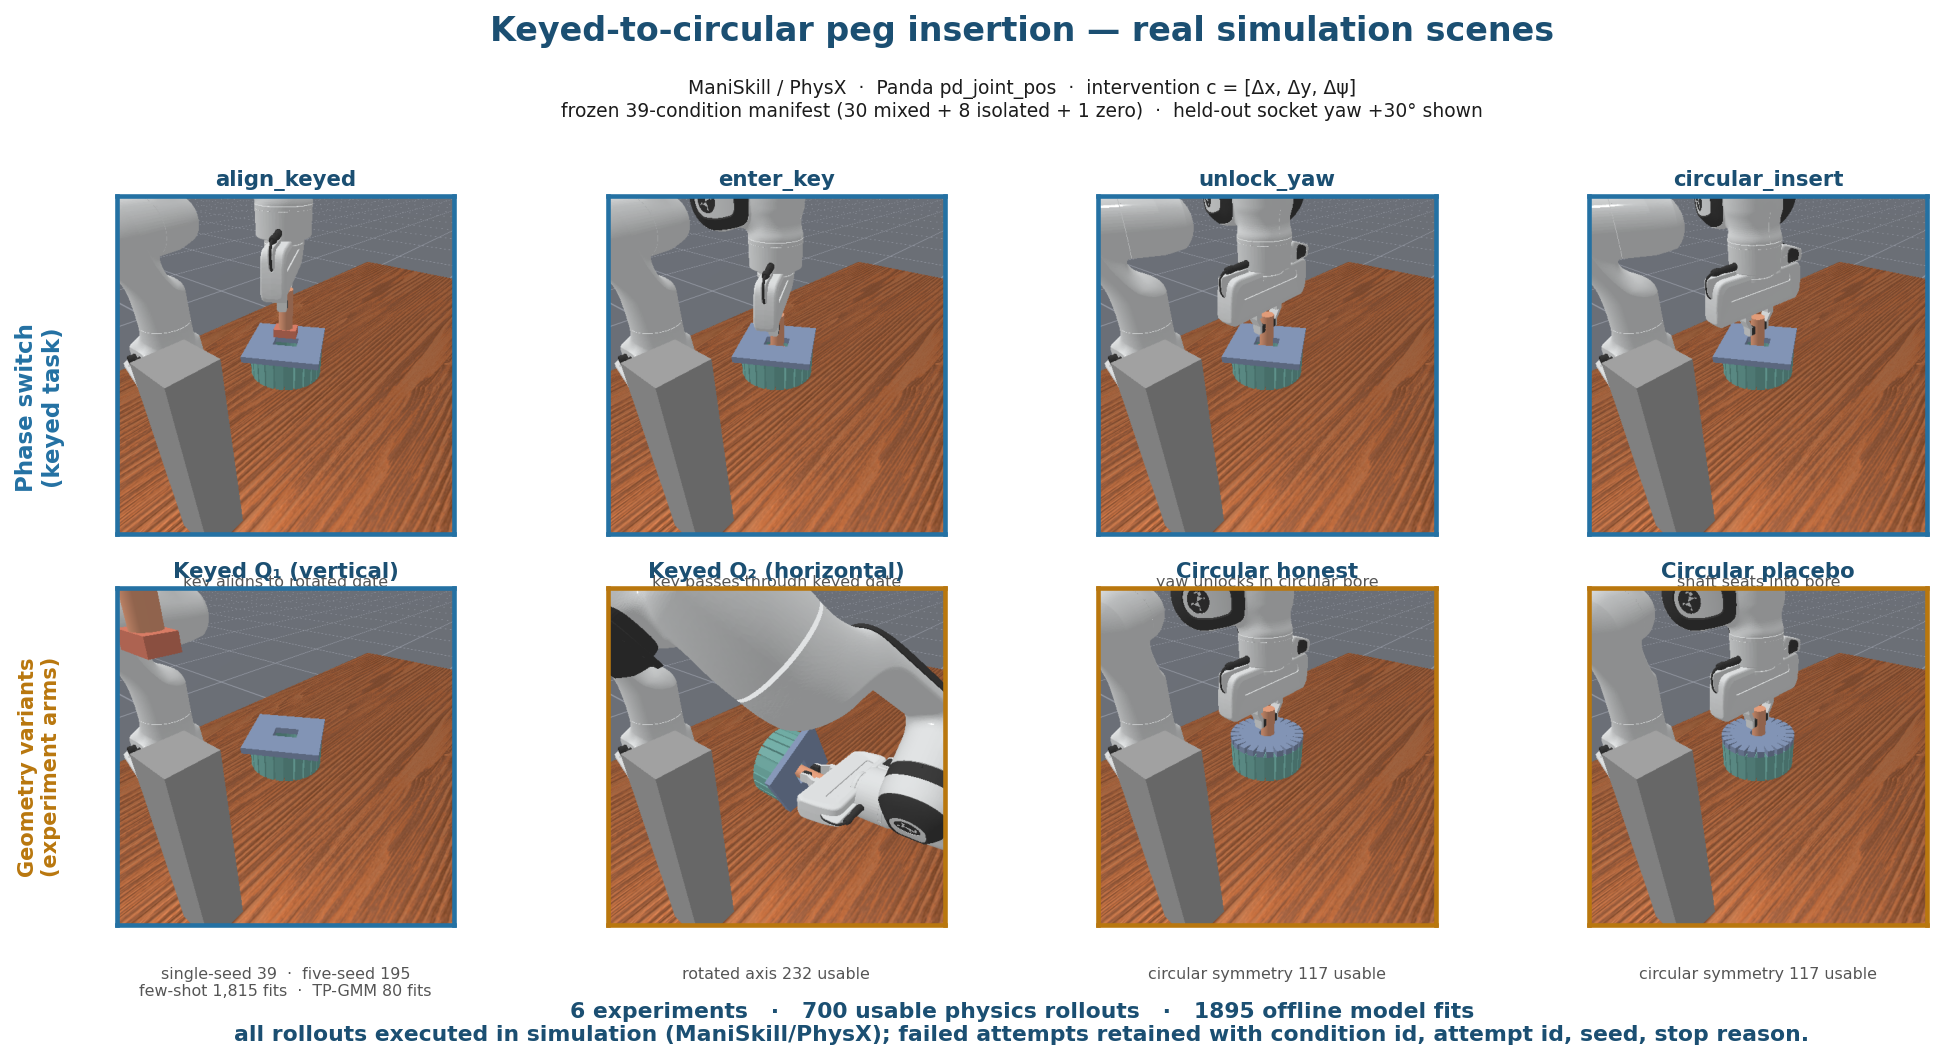
\includegraphics[width=\columnwidth,trim=0 52 0 0,clip]{experiment_overview_scenes.png}
    \caption{Experimental controls. The same generator coordinate
    $\Delta\psi$ is relevant in the keyed entry phase, irrelevant after
    clearance, and a pure gauge in the circular honest/placebo arms.}
    \label{fig:overview_scenes}
\end{figure}

\section{Results}
\label{sec:results}

\subsection{The Phase Switch Is Physically Expressed}

The single-seed task validates the core mechanism before any model comparison.
Translation remains relevant to the endpoint, yaw is relevant immediately
before key clearance, and yaw is suppressed after the task enters the circular
bore. The isolated-response checks are summarized in
Table~\ref{tab:physics}. The learned final response is approximately
$\mathrm{Diag}(1.0024,1.0000,-0.00031)$, while the best scalar frame weight is
$w=0.5681$, illustrating the compromise predicted by
Eq.~\eqref{eq:best_scalar}.

\begin{table}[t]
\centering
\caption{Strict single-seed physics validation. Ratios are empirical isolated
generator responses.}
\label{tab:physics}
\small
\setlength{\tabcolsep}{4.0pt}
\begin{tabular}{lcc}
\toprule
Check & Criterion & Result\\
\midrule
Final translation & $\geq0.8$ & 0.9872\\
Pre-clear yaw & $\geq0.8$ & 0.9997\\
Unlock yaw & $\leq0.25$ & 0.0028\\
Final yaw & $\leq0.25$ & 0.0022\\
Scalar $\rightarrow P_{\rm diag}$ endpoint & lower & 6.554 $\rightarrow$ 0.639\\
Pairwise contact in usable data & present & 2 episodes\\
\bottomrule
\end{tabular}
\end{table}

\subsection{Strong Baselines Confirm the Frame-Level Failure}

Table~\ref{tab:baseline} reports the frozen strong-baseline benchmark on the
same train/test split. Scalar frame relevance and the phase scalar GP preserve a
single frame-level weight and therefore cannot keep translation near one while
suppressing final yaw. TP-GMM and generic/dense regressors recover the switch
better, showing that anisotropic behavior is possible without our
parameterization. The smooth finite $P_{\rm diag}$ model is not uniformly the
lowest-error predictor, but it preserves the intended law with a constrained,
interpretable finite-action operator.

\begin{table*}[t]
\centering
\caption{Held-out baseline benchmark on the frozen single-seed dataset. Errors
are mean mm-equivalent values; switch error is measured against the isolated
half-decay target.}
\label{tab:baseline}
\small
\setlength{\tabcolsep}{4.2pt}
\begin{tabular}{lcccccc}
\toprule
Model & Task traj. & Endpoint & Gen. RMSE & Final trans. & Pre-yaw & Final yaw\\
\midrule
Frame-weighted & 4.765 & 3.262 & 0.354 & 0.568 & 1.004 & 0.568\\
Phase scalar GP & 4.764 & 3.261 & 0.354 & 0.568 & 1.004 & 0.568\\
TP-GMM SE(2) & 4.159 & 0.298 & 0.177 & 0.998 & 0.946 & 0.0018\\
Generic RBF & \textbf{3.316} & \textbf{0.251} & 0.196 & 1.001 & 1.000 & -0.0003\\
Full operator & 3.304 & \textbf{0.251} & 0.196 & 1.001 & 1.000 & -0.0003\\
$P_{\rm diag}$ finite & 3.448 & 0.427 & 0.192 & 0.985 & 1.000 & 0.0258\\
\bottomrule
\end{tabular}
\end{table*}

\begin{figure}[t]
    \centering
    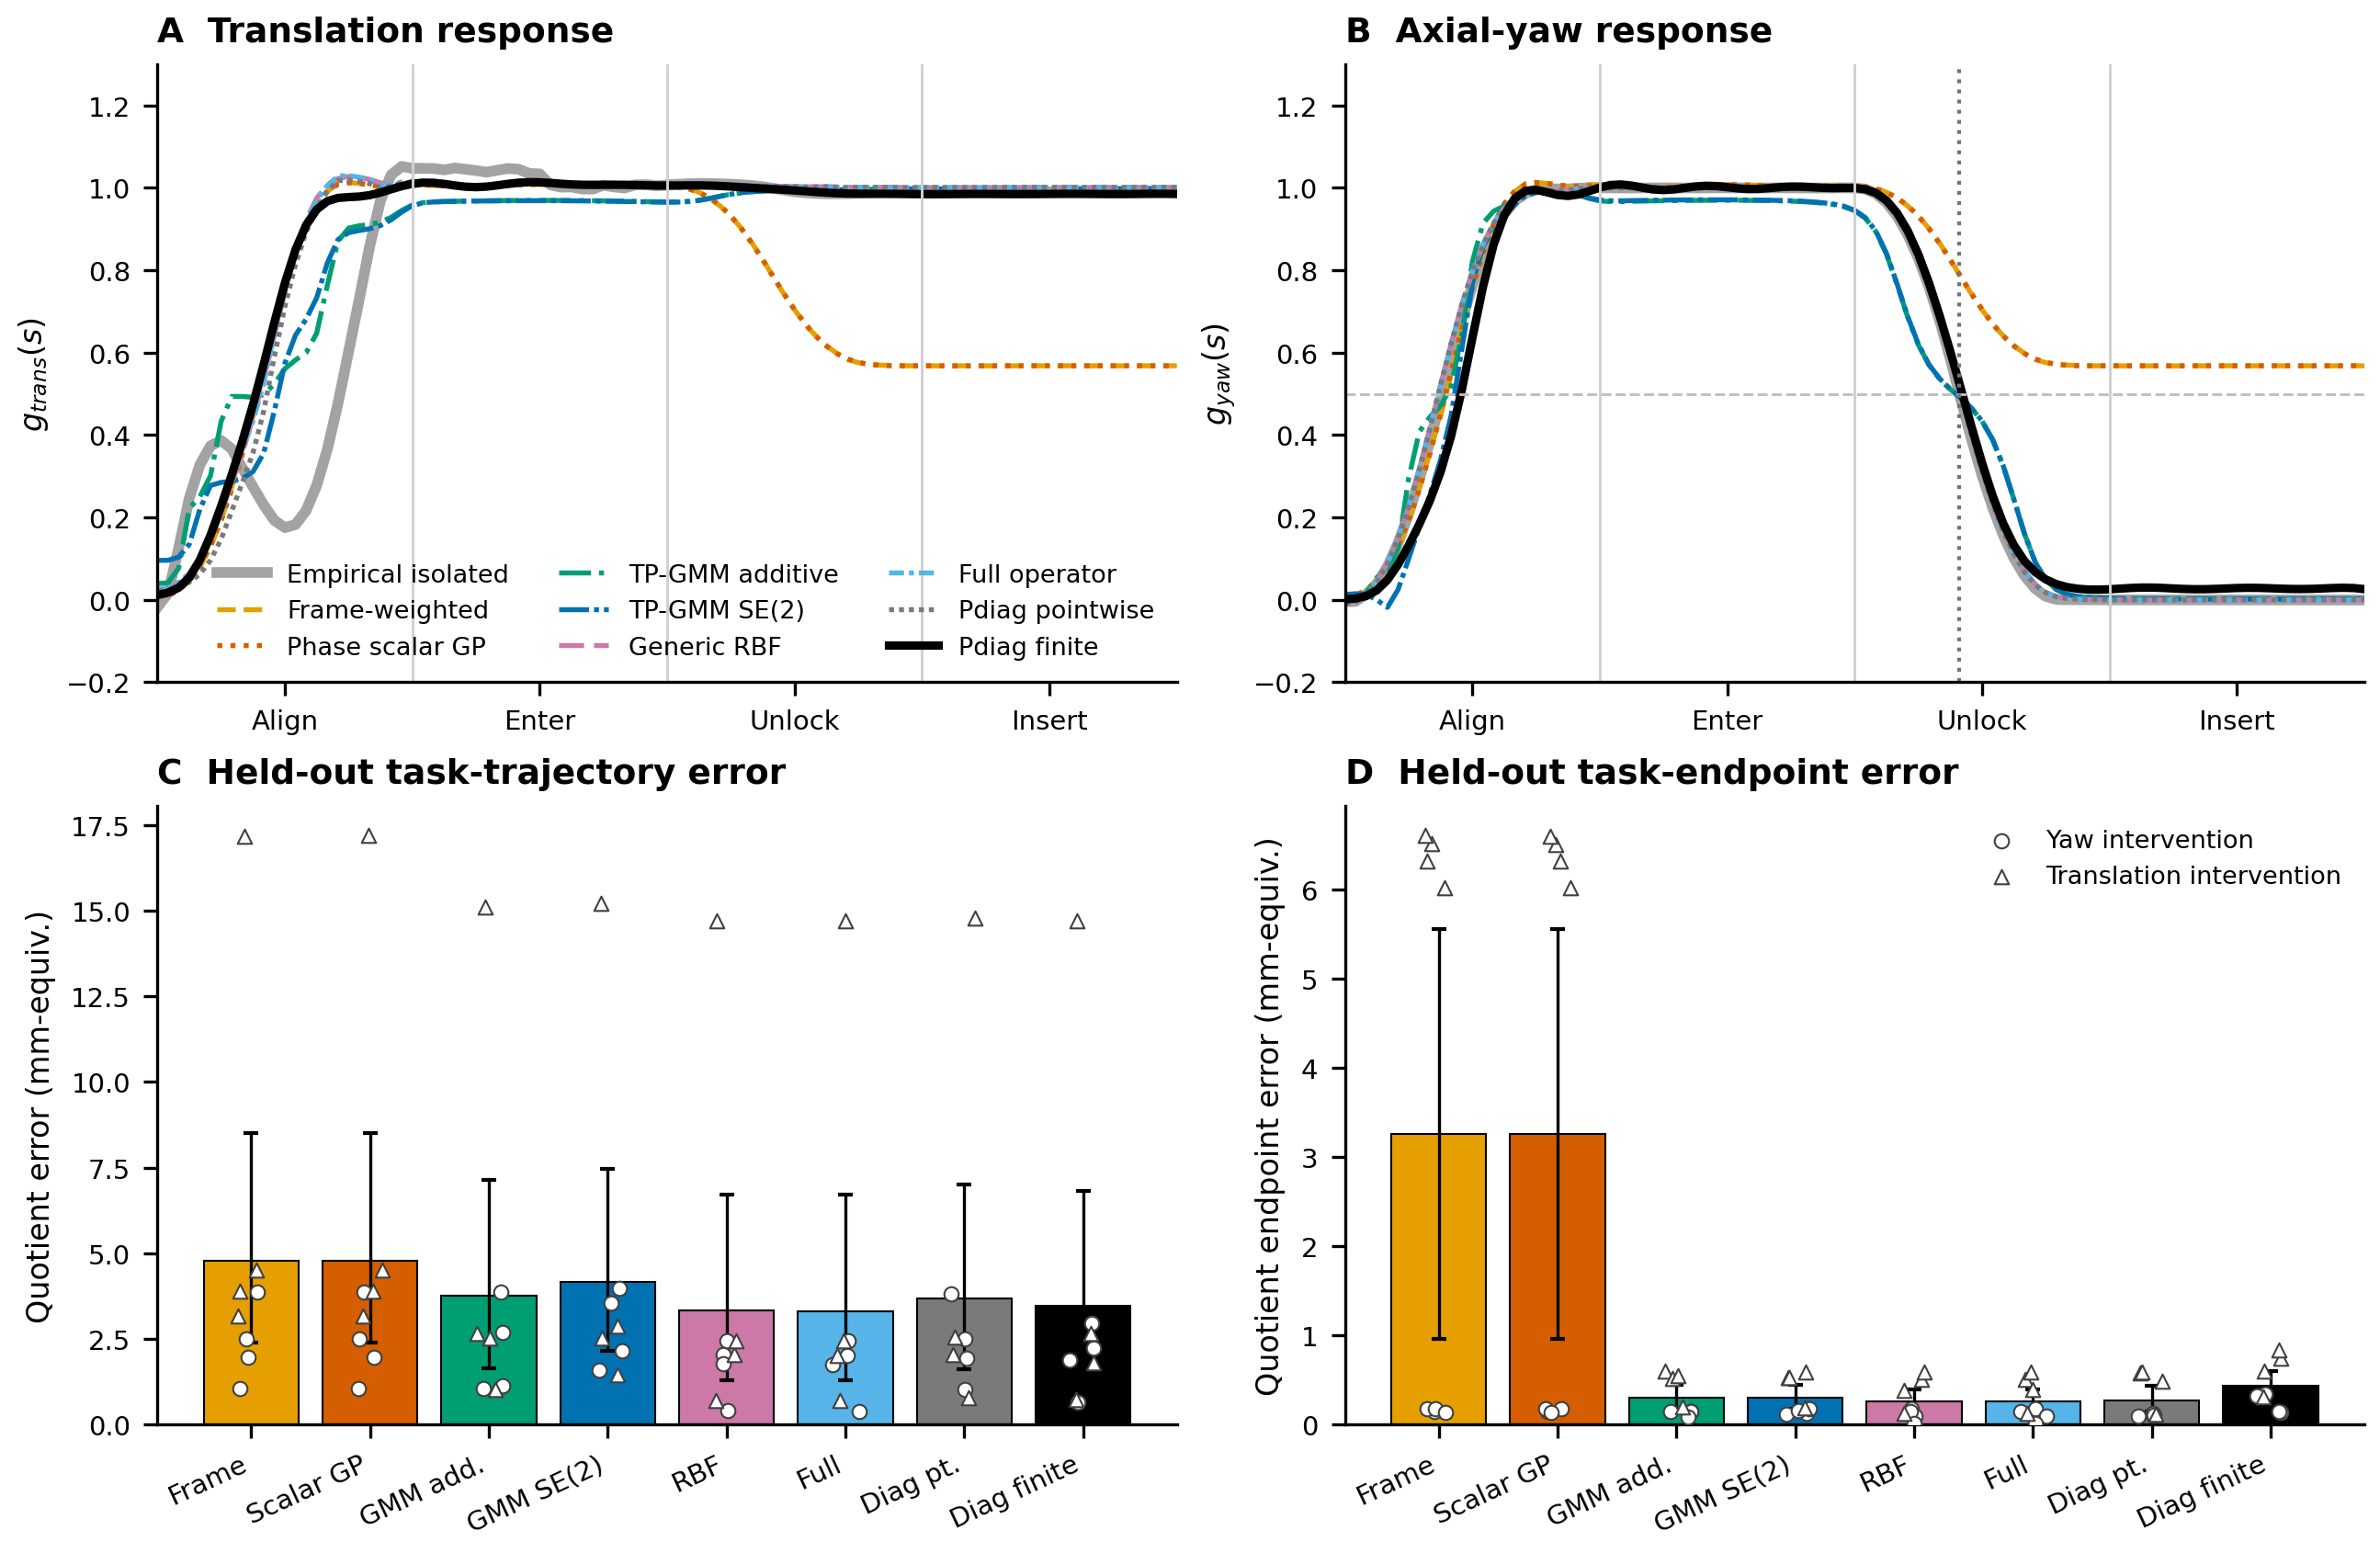
\includegraphics[width=\columnwidth]{phase_switch_symmetry_baselines/phase_switch_strong_baselines.png}
    \caption{Strong-baseline profiles and held-out errors on the frozen
    single-seed phase-switch dataset.}
    \label{fig:baseline}
\end{figure}

\subsection{The Law Replicates Across Seeds and Few-Shot Subsets}

All five fixed-context seeds satisfy the preregistered criteria
(Table~\ref{tab:multiseed}). The mean scalar-minus-$P_{\rm diag}$ task-error
improvement is $1.7576\pm0.4653$\,mm-equivalent across seeds, with a
seed-then-condition bootstrap interval of $[1.2964,2.2295]$.

\begin{table}[t]
\centering
\caption{Five independent fixed-context fits.}
\label{tab:multiseed}
\small
\setlength{\tabcolsep}{3.5pt}
\begin{tabular}{lcccc}
\toprule
Seed & Final trans. & Pre-yaw & Final yaw & $E_{\rm task}$\\
\midrule
20260818 & 0.9847 & 0.9983 & 0.0234 & 2.1360\\
20270818 & 0.9972 & 0.9966 & 0.0273 & 2.1908\\
20280818 & 0.9875 & 0.9985 & 0.0250 & 3.4594\\
20290818 & 0.9821 & 0.9959 & 0.0251 & 2.5222\\
20300818 & 0.9797 & 0.9999 & 0.0283 & 1.6195\\
\bottomrule
\end{tabular}
\end{table}

In the repeated few-shot sweep, $P_{\rm diag}$ detects the switch in all subsets
at every sample size. Its complete generator-law pass rate is 88\% for random
$N=3$, 92\% for qualified $N=3$, and 100\% for both protocols at every
$N\geq5$. The matched TP-GMM few-shot experiment is summarized in
Table~\ref{tab:fewshot_tpgmm}; $P_{\rm diag}$ wins every matched seed/subset
cell at each tested $N$.

\begin{table}[t]
\centering
\caption{Matched few-shot task-trajectory error against rotation-aware
TP-GMM SE(2). Values are means over matched seed/subset cells.}
\label{tab:fewshot_tpgmm}
\small
\setlength{\tabcolsep}{4.2pt}
\begin{tabular}{lcccc}
\toprule
$N$ & $P_{\rm diag}$ & TP-GMM SE(2) & Full op. & RBF\\
\midrule
5 & \textbf{2.71} & 7.58 & 4.11 & 5.91\\
10 & \textbf{2.67} & 4.43 & 3.94 & 5.27\\
20 & \textbf{2.43} & 3.78 & 3.28 & 4.02\\
30 & \textbf{2.39} & 3.46 & 3.07 & 3.63\\
\bottomrule
\end{tabular}
\end{table}

\begin{figure}[t]
    \centering
    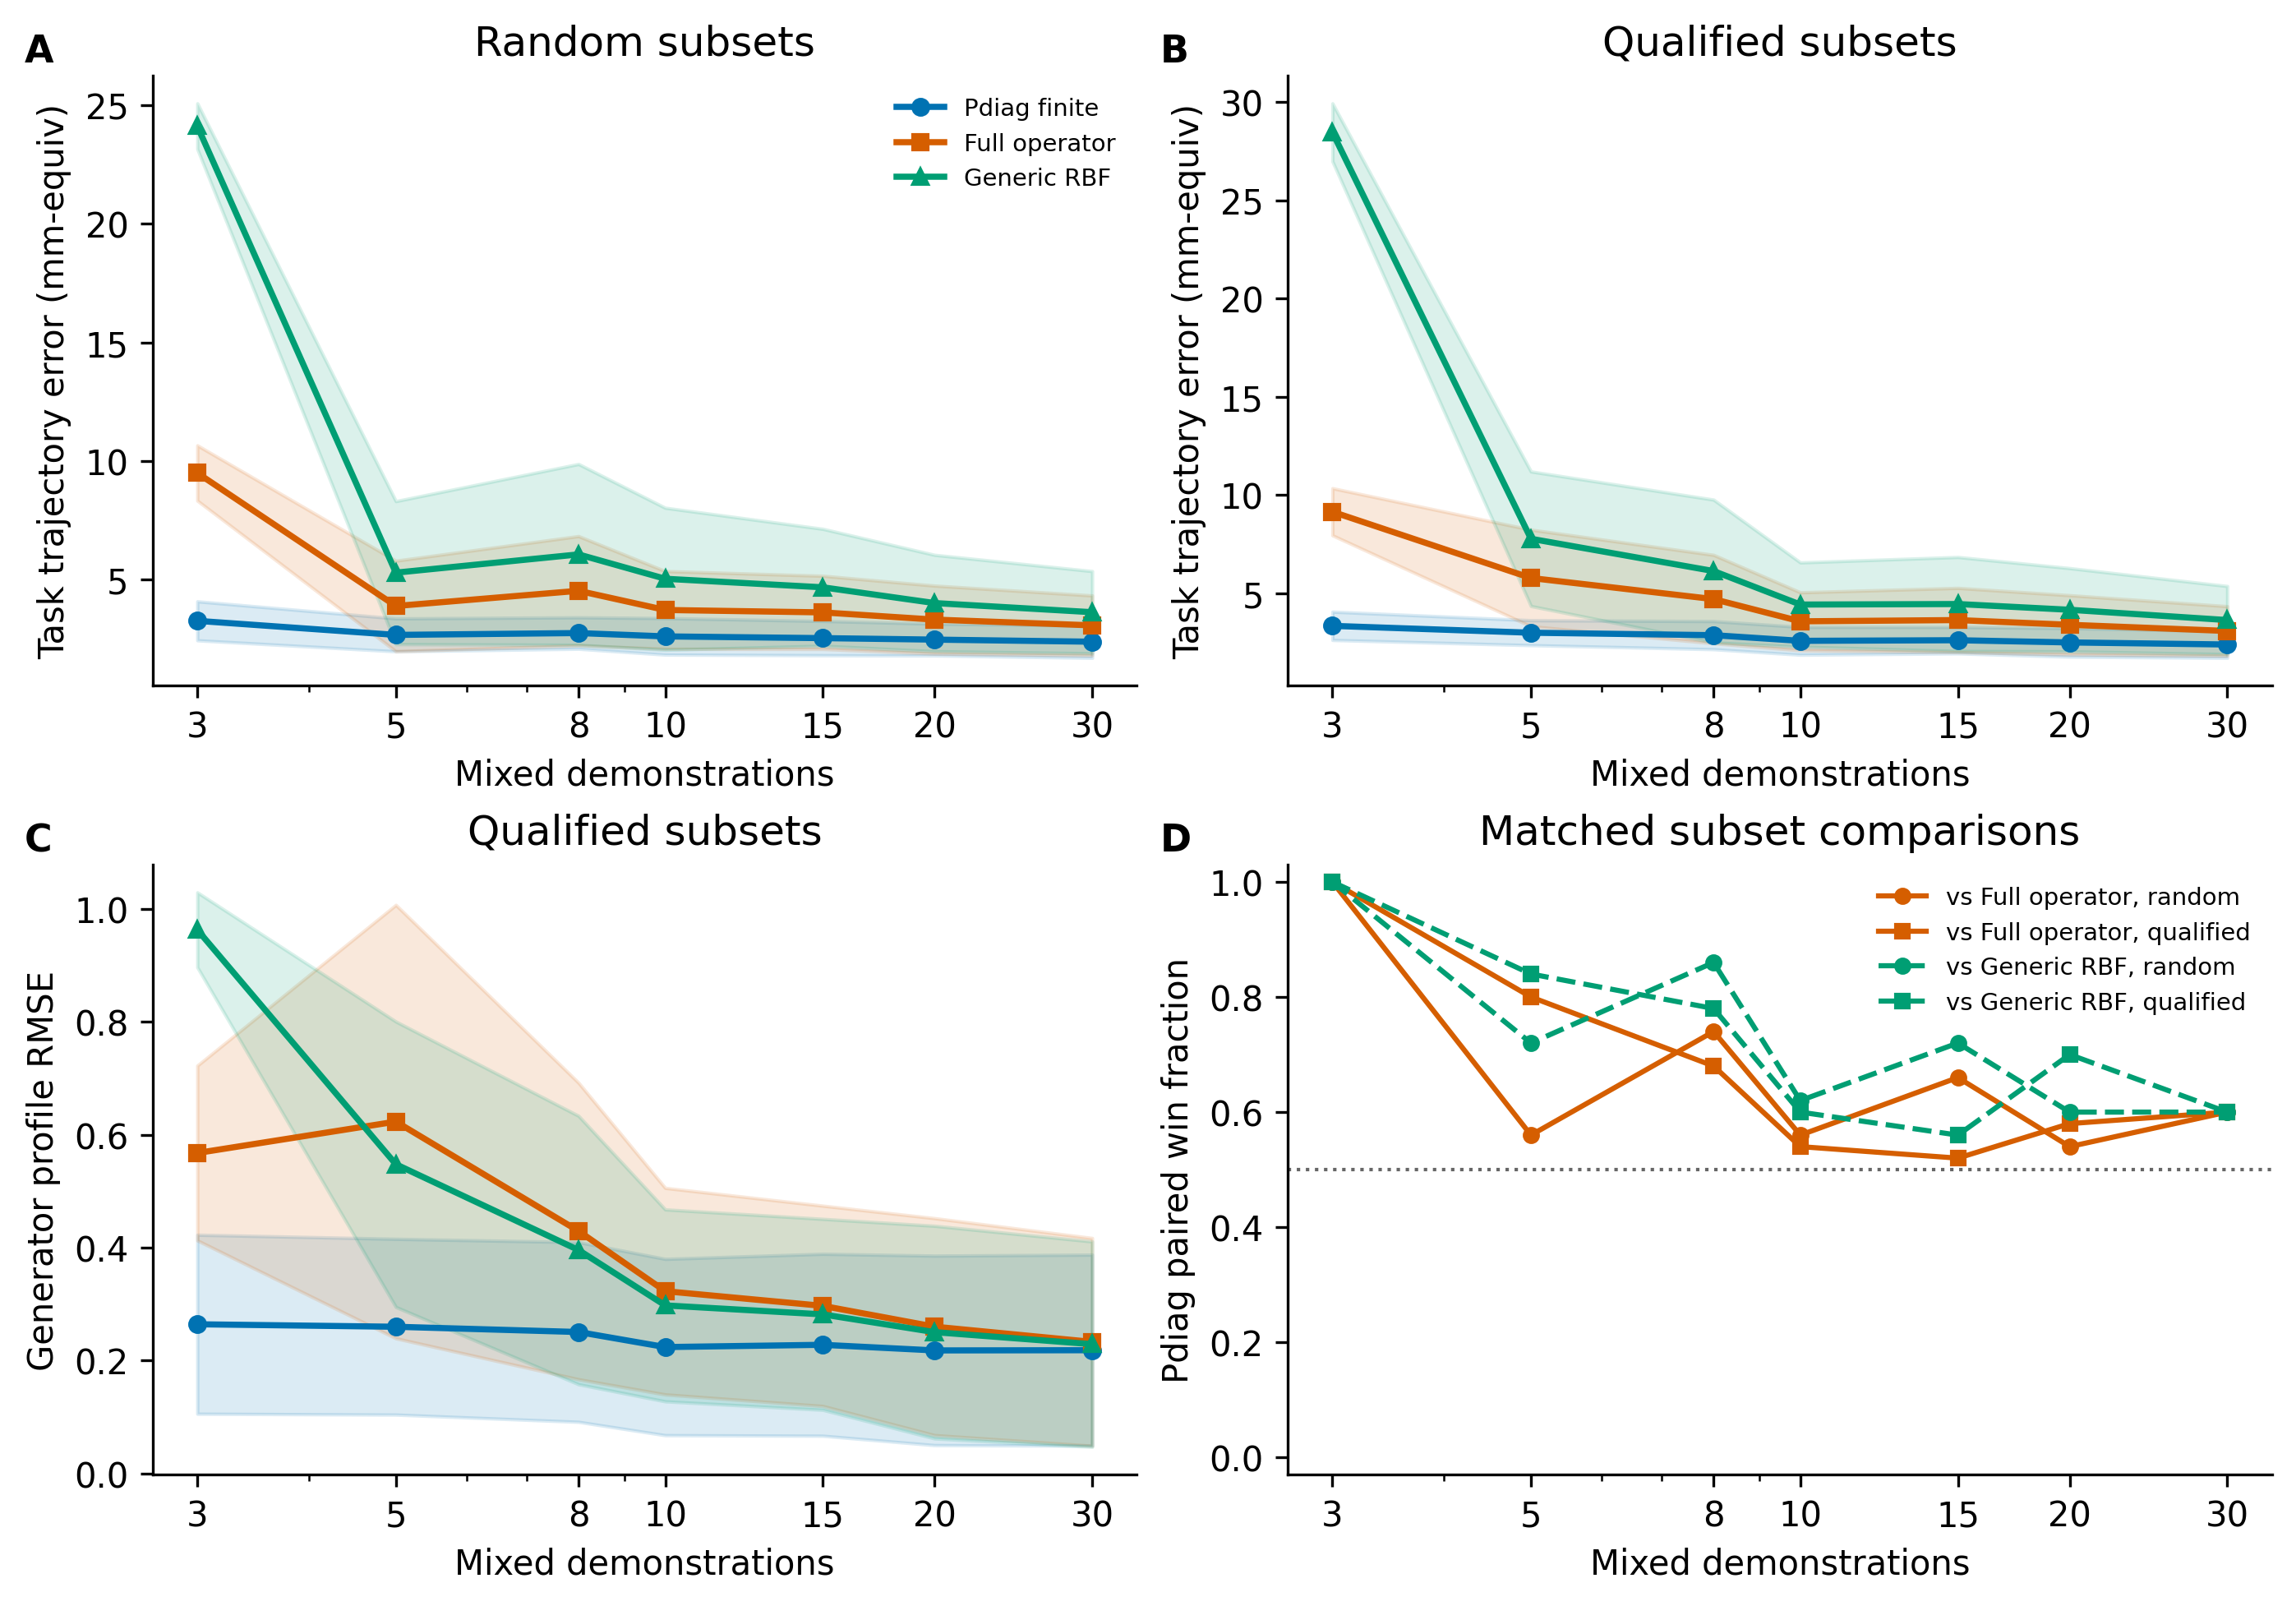
\includegraphics[width=\columnwidth]{phase_switch_symmetry_multiseed/fewshot_results/phase_switch_fewshot.png}
    \caption{Few-shot recovery over fixed seed/subset cells. The structured
    diagonal finite-action model is most valuable in the low-sample regime.}
    \label{fig:fewshot}
\end{figure}

\subsection{Privileged Phase Labels Are Not Required}

Non-oracle progress experiments show that the recovered law is not an artifact
of using solver phase labels. Normalized time is poor; observable geometric
progress is substantially better. Offline DTW-position is the strongest upper
bound because it uses the full sequence for alignment, and therefore should not
be interpreted as a deployable estimator.

\begin{table}[t]
\centering
\caption{Physical-timeline non-oracle progress results, averaged over five
seeds. $dE$ is relative to the oracle semantic-phase reference.}
\label{tab:nonoracle}
\small
\setlength{\tabcolsep}{4.0pt}
\begin{tabular}{lccc}
\toprule
Progress & $E_{\rm task}^{\rm phys}$ & $dE$ & $E_{\rm gen}$\\
\midrule
Oracle phase & 4.60 & 0.00 & 0.218\\
Time & 11.11 & +6.50 & 0.745\\
Arc length & 5.50 & +0.90 & 0.328\\
Keypoint & 8.89 & +4.29 & 0.349\\
DTW-position & \textbf{3.19} & -1.42 & \textbf{0.130}\\
\bottomrule
\end{tabular}
\end{table}

\subsection{The Generator Law Is Task-Local}

The rotated-axis experiment tests whether the model merely learned a world-yaw
heuristic. After canonicalizing by the inverse global task rotation, the axial
profile is highly consistent between vertical Q1 and horizontal Q2 executions
(Table~\ref{tab:rotated}). Because Q2's axial generator is not world yaw, this
supports the task-local interpretation. One Q1 seed falls below the
translation threshold, but the axial law is preserved in all matched seeds.

\begin{table}[t]
\centering
\caption{Matched Q1/Q2 rotated-axis consistency.}
\label{tab:rotated}
\small
\setlength{\tabcolsep}{4.2pt}
\begin{tabular}{lccc}
\toprule
Seed & $D_{\rm orient}$ & $\rho_{\rm axial}$ & $|d g_{\psi}^{\rm final}|$\\
\midrule
20260818 & 0.112 & 0.985 & 0.015\\
20270818 & 0.289 & 0.941 & 0.005\\
20280818 & 0.148 & 0.938 & 0.004\\
\bottomrule
\end{tabular}
\end{table}

\subsection{Symmetry Intervention: Relation Rather Than Trajectory Statistics}

The circular symmetry intervention closes the main causal chain. Step 0 first
validates the geometry: nominal circular insertion succeeds, and the isolated
axial-yaw slope at alignment is 0.0000, confirming that $\Delta\psi$ is a gauge
intervention before any benchmark fitting. All nine datasets
(3 arms $\times$ 3 seeds) then realize 39/39 usable condition cells. The scored
benchmark has 1296 fits and zero failures.

\begin{figure*}[t]
    \centering
    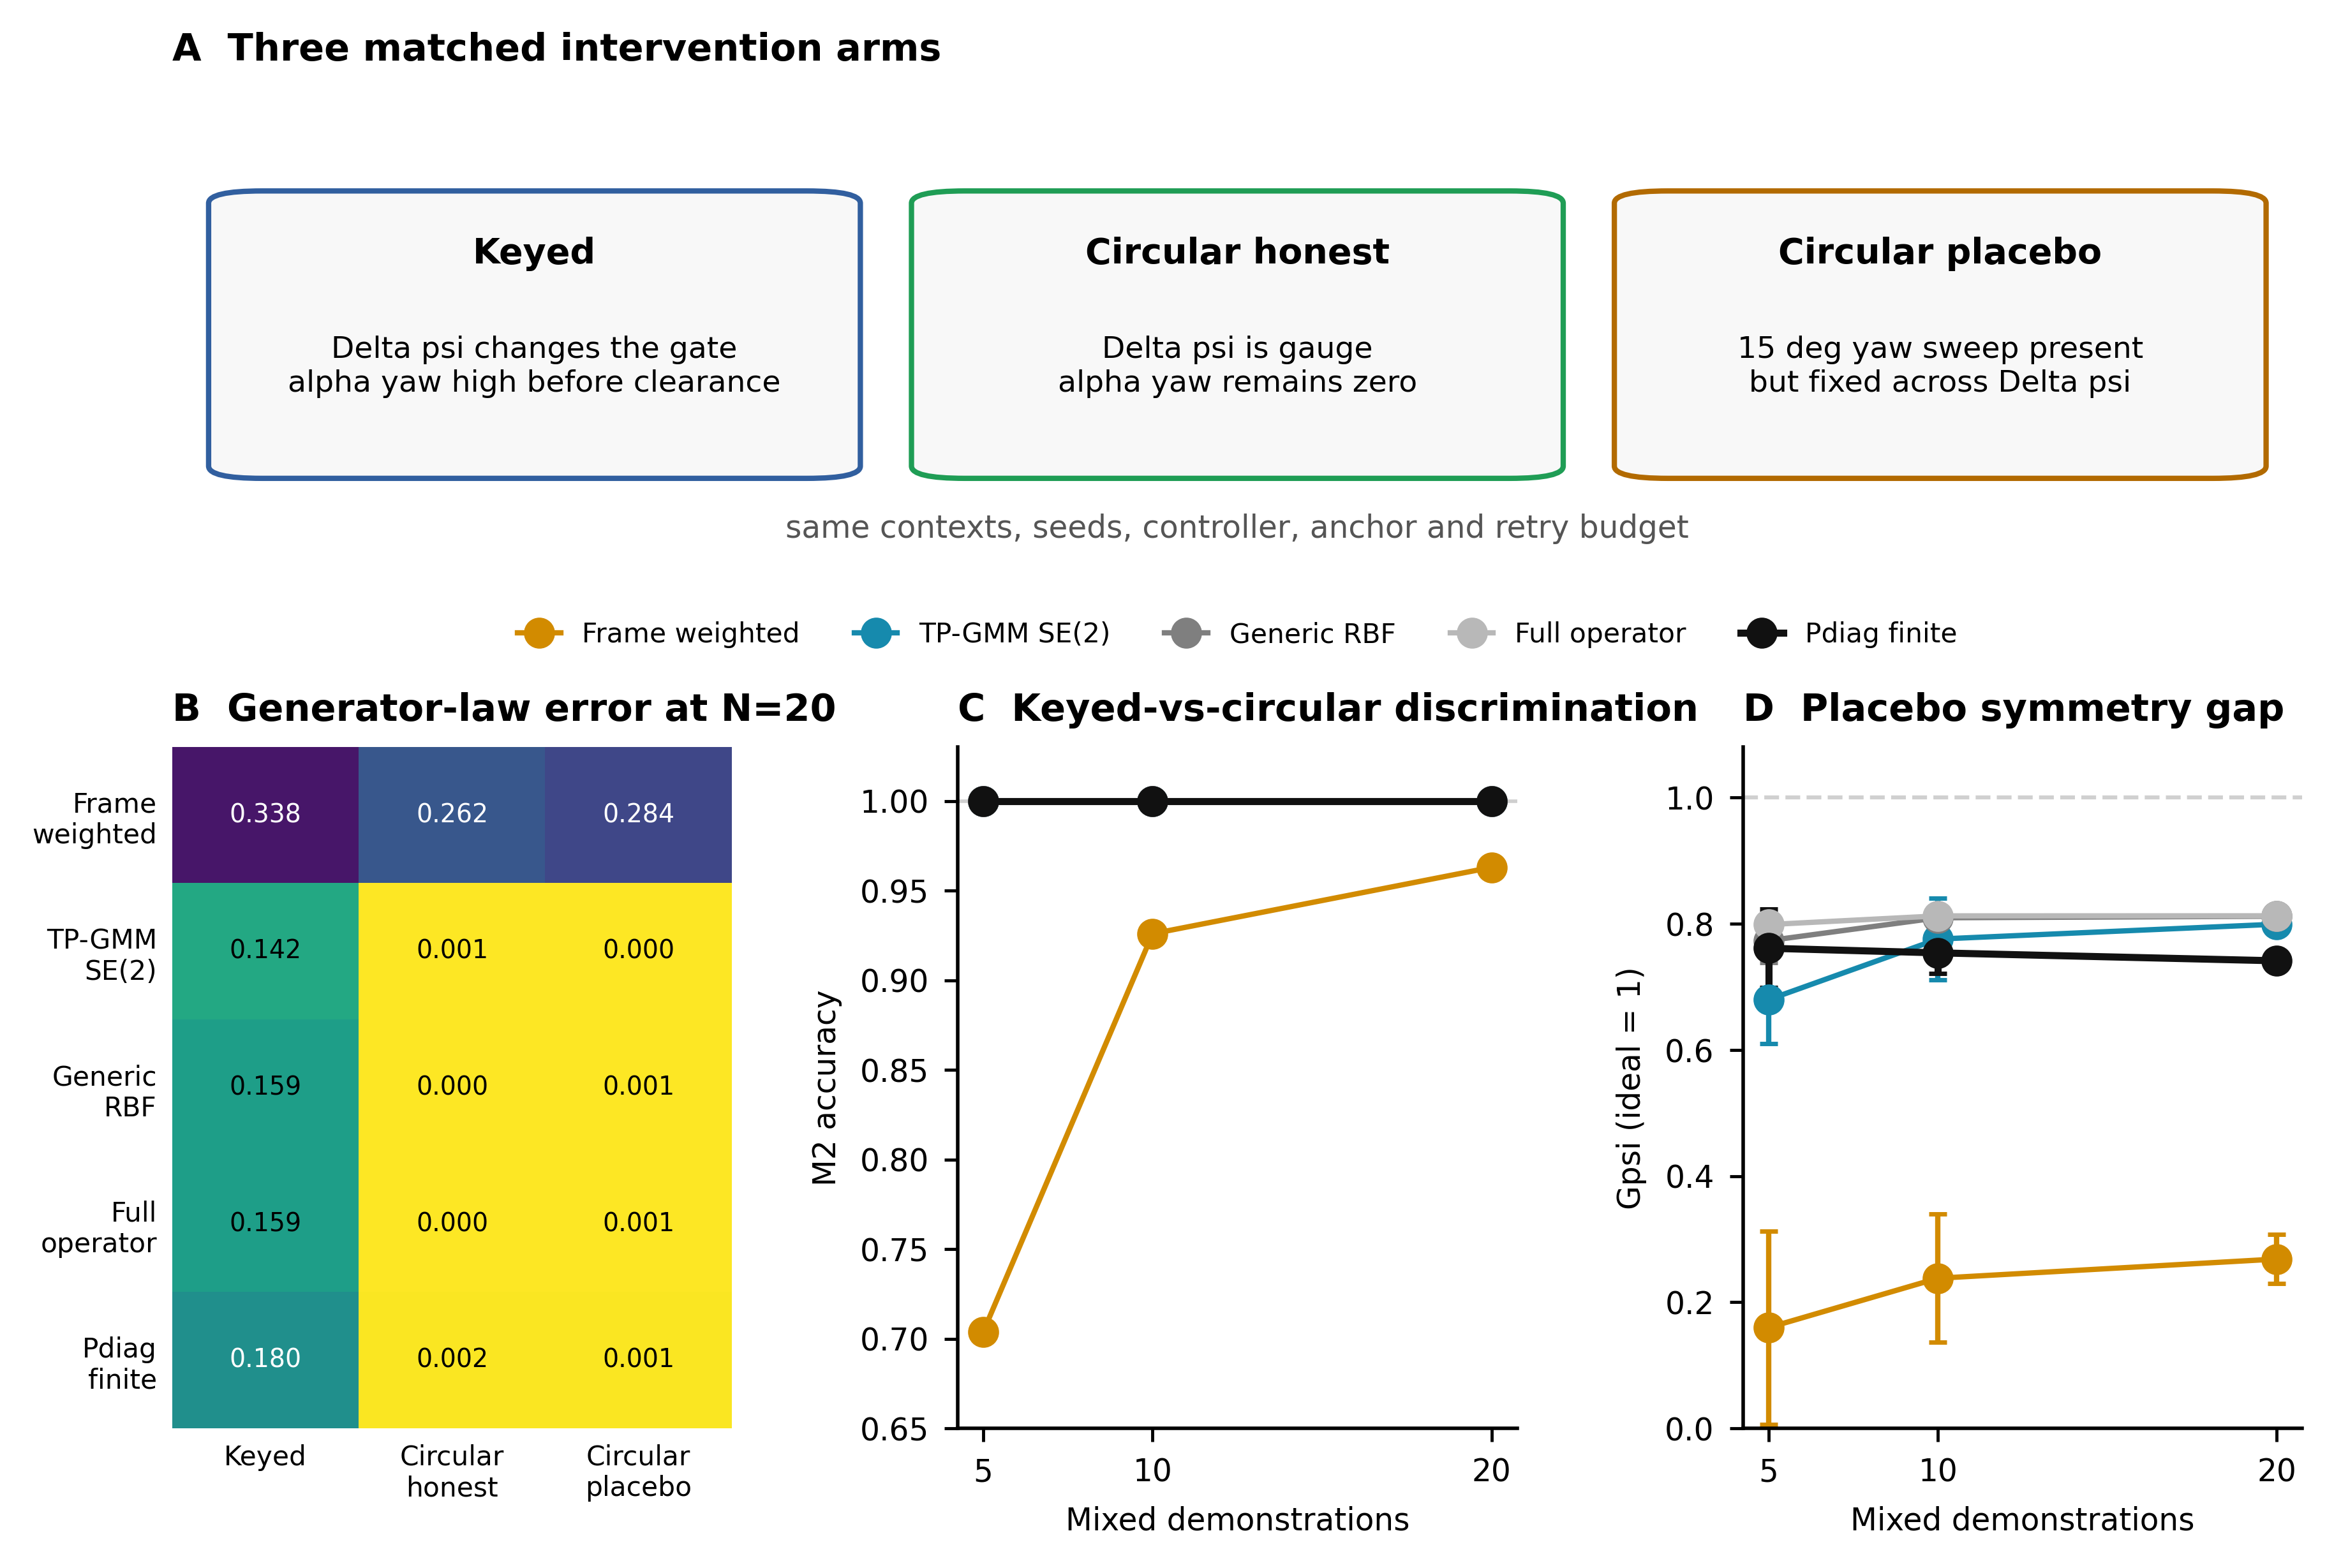
\includegraphics[width=\textwidth]{symmetry_transfer_main.png}
    \caption{Causal symmetry-transfer benchmark. A, The keyed, circular-honest,
    and circular-placebo arms share contexts, seeds, controller, anchor, and
    retry budget; the placebo arm contains yaw motion that is fixed across
    axial-yaw interventions. B, M1 generator-law error at $N=20$ separates
    scalar frame baselines from relational or structured models on circular
    arms. C, M2 keyed-vs-circular discrimination is perfect for finite
    $P_{\rm diag}$ down to $N=5$, while scalar frame baselines improve only
    with more demonstrations. D, The placebo symmetry gap shows that the fixed
    yaw sweep does not create yaw relevance for relational models.}
    \label{fig:symmetry_transfer}
\end{figure*}

Figure~\ref{fig:symmetry_transfer} and Table~\ref{tab:sym_m1} report M1 at
$N=20$. On both circular arms, every
relational or structured model reads $\alpha_\psi\approx0$; the finite
$P_{\rm diag}$ errors are 0.0016 on honest and 0.0015 on placebo. The two
marginal frame-level baselines hallucinate yaw relevance on the circular arms
($E_\alpha\approx0.26$--0.28), because a scalar frame response cannot separate
the relevant translations from the irrelevant axial generator. The keyed arm is
harder because the oracle has a sharp phase boundary; smooth models place the
drop around the physical release rather than at an instantaneous boundary.
The finite $P_{\rm diag}$ switch diagnostic M0 nevertheless detects the keyed
phase change in 100\% of fits at $N=5,10,20$, with mean switch locations
0.606, 0.608, and 0.608 on normalized progress.

\begin{table*}[t]
\centering
\caption{Symmetry-intervention generator identification error M1 at $N=20$.
Lower is better. The placebo arm contains a fixed yaw sweep in the trajectory
but zero response to the axial-yaw intervention.}
\label{tab:sym_m1}
\small
\setlength{\tabcolsep}{5.0pt}
\begin{tabular}{lccc}
\toprule
Model & Keyed & Circular honest & Circular placebo\\
\midrule
Frame-weighted & 0.338 & 0.262 & 0.284\\
Phase scalar GP & 0.338 & 0.262 & 0.284\\
TP-GMM additive & \textbf{0.132} & 0.0006 & 0.0005\\
TP-GMM SE(2) & 0.142 & 0.0006 & \textbf{0.0004}\\
Generic RBF & 0.159 & \textbf{0.00008} & 0.0006\\
Full operator & 0.159 & 0.0002 & 0.0006\\
$P_{\rm diag}$ pointwise & 0.158 & 0.0001 & 0.0005\\
$P_{\rm diag}$ finite & 0.180 & 0.0016 & 0.0015\\
\bottomrule
\end{tabular}
\end{table*}

The headline discrimination metric M2 classifies a fit as keyed iff
$\alpha_\psi^{\rm pre}>0.5$. The finite $P_{\rm diag}$ model is correct on
100\% of fits down to $N=5$, as are the full operator, pointwise diagonal,
generic RBF, and TP-GMM SE(2). TP-GMM additive reaches 96.3\% at $N=5$ and
100\% at $N\geq10$. In contrast, frame-weighted and phase-scalar GP baselines
remain below 100\% even at $N=20$ (70.4\%, 92.6\%, 96.3\% for
$N=5,10,20$). Thus the intervention is identifiable from few demonstrations,
but not uniquely by our model; the distinctive role of $P_{\rm diag}$ is the
explicit generator prior and few-shot reliability.

\begin{table}[t]
\centering
\caption{Placebo symmetry gap
$G_\psi=\alpha_\psi^{\rm pre}(\mathrm{keyed})-
\alpha_\psi^{\rm pre}(\mathrm{circular\ placebo})$. The ideal value is 1.}
\label{tab:sym_gap}
\small
\setlength{\tabcolsep}{4.0pt}
\begin{tabular}{lccc}
\toprule
Model & $N=5$ & $N=10$ & $N=20$\\
\midrule
Frame-weighted & 0.160 & 0.238 & 0.268\\
Phase scalar GP & 0.160 & 0.238 & 0.268\\
TP-GMM additive & 0.627 & 0.782 & 0.790\\
TP-GMM SE(2) & 0.680 & 0.776 & 0.799\\
Generic RBF & 0.773 & 0.809 & 0.812\\
Full operator & 0.799 & 0.813 & 0.813\\
$P_{\rm diag}$ pointwise & \textbf{0.814} & \textbf{0.815} & \textbf{0.813}\\
$P_{\rm diag}$ finite & 0.761 & 0.754 & 0.741\\
\bottomrule
\end{tabular}
\end{table}

Table~\ref{tab:sym_gap} shows the placebo contrast directly. The relational
models produce large gaps, while the marginal baselines remain near 0.16--0.27.
The gap falls short of the ideal value 1 because the keyed pre-clear mean
relevance saturates around 0.75--0.81 over the whole pre-insertion window rather
than staying exactly at 1; the smooth finite model intentionally spreads the
transition over progress. The point is not that $P_{\rm diag}$ finite maximizes
this location statistic, but that it assigns the same near-zero yaw relevance
to honest and placebo circular arms despite the placebo trajectory containing
rotation.

The reliability analysis explains why the constrained generator prior remains
useful when flexible models also identify the relation. On the hardest
few-shot circular-honest case ($N=5$), the full operator has mean
$E_\alpha=0.062$ with total standard deviation 0.253 and one catastrophic
hallucination out of 18 cells ($E_\alpha=1.106$). The finite $P_{\rm diag}$
has mean $E_\alpha=0.0077$, total standard deviation 0.011, worst case 0.045,
and zero hallucinations. The generic RBF is also stable on this diagnostic
($E_\alpha=0.0003$, worst case 0.0020), so the correct claim is not exclusive
accuracy, but that the diagonal finite-action prior removes the fat overfitting
tail of an unconstrained operator while preserving an interpretable generator
law.

\begin{table}[t]
\centering
\caption{Few-shot stability on the circular-honest arm at $N=5$. Hallucination
denotes fits whose circular yaw relevance exceeds the preregistered threshold.}
\label{tab:sym_var}
\small
\setlength{\tabcolsep}{4.0pt}
\begin{tabular}{lcccc}
\toprule
Model & Mean & Std. & Worst & Halluc.\\
\midrule
Frame-weighted & 0.300 & 0.063 & 0.404 & 1.000\\
Full operator & 0.062 & 0.253 & 1.106 & 0.056\\
Generic RBF & \textbf{0.0003} & \textbf{0.0006} & \textbf{0.002} & 0.000\\
$P_{\rm diag}$ finite & 0.0077 & 0.011 & 0.045 & 0.000\\
\bottomrule
\end{tabular}
\end{table}

Finally, M3 confirms that honest and placebo are behaviorally distinct even
though both have $\alpha_\psi=0$: at $N=20$, a finite-$P_{\rm diag}$ model fit
on circular-honest incurs an additional 8.89 mm-equivalent error when evaluated
on circular-placebo, and the reverse gap is 8.46. Thus the benchmark separates
marginal trajectory shape from intervention response: the placebo arm contains
yaw motion, but the learned generator relevance remains zero because that
motion is uncorrelated with $\Delta\psi$.

\section{Discussion}
\label{sec:discussion}

\subsection{What the Evidence Shows}

The completed experiments support the central structural claim. A scalar
frame-level relevance is forced to compromise: it can preserve translation or
suppress yaw, but not both when the same relation has
$\mathrm{Diag}(1,1,0)$ relevance. The single-seed physics validation shows this
law in isolated interventions; the strong-baseline benchmark shows that the
failure is structural for scalar frame relevance; the circular honest/placebo
intervention rejects the alternative that the method is merely detecting
rotation in the trajectory; and the five-seed/few-shot replications show that
the diagonal finite-action model identifies the law from few mixed
demonstrations.

The results do not show that $P_{\rm diag}$ is the most accurate possible
predictor. Generic RBF and full operators are competitive on full-data
single-seed error, and TP-GMM SE(2) is a meaningful rotation-aware baseline.
The proposed advantage is instead interpretability and sample efficiency: the
learned object is a generator law that can be inspected directly, tied to task
symmetry, and stress-tested under isolated interventions.

\subsection{Task Equivalence versus Robot Realization}

The quotient metric is necessary because post-clear axial yaw is task
equivalent for the circular bore. Penalizing arbitrary axial spin would measure
planner or inverse-kinematics realization rather than insertion error. At the
same time, quotient evaluation alone would be insufficient: a method could
achieve low task error while propagating an irrelevant yaw generator. The
combination of isolated generator-law recovery and quotient task-space error is
therefore essential.

\subsection{Limitations and Open Edges}

The current causal study isolates a three-generator subgroup $(x,y,\psi)$
rather than the full six-dimensional $SE(3)$ relation. Extending the approach
to full 6-DoF manipulation requires physically meaningful generator bases and
excitation checks in all claimed directions. The controlled ManiSkill/PhysX
experiments are designed to isolate the generator law under fixed contexts,
controllers, and seeds; the corresponding hardware study should preserve the
same three-arm intervention logic and report the same generator-law metrics
rather than replacing the claim with a raw success-rate comparison.

The circular honest/placebo intervention is the strongest current evidence
because it changes task symmetry while preserving the surrounding execution
pipeline. The placebo arm is especially important: it contains a visible yaw
sweep in the trajectory, yet this sweep is fixed across axial-yaw interventions.
Models that learn the intervention-response relation therefore assign
$\alpha_\psi\approx0$, while frame-level baselines still leak yaw relevance
from the frame change. This closes the main alternative explanation that the
method is only detecting whether rotation appears in the motion.

\section{Conclusion}
\label{sec:conclusion}

Task frames can be too coarse a unit for geometric skill generalization. A
frame bundles multiple geometric generators, but a manipulation skill may need
to follow some of them, ignore others, and change this behavior with task
progress. The proposed phase-dependent diagonal operator makes this granularity
explicit and separates learned task relevance from finite rigid-body
realization. In the keyed-to-circular insertion benchmark, it recovers a
physically grounded transition from yaw-relevant keyed entry to yaw-invariant
circular insertion, while preserving lateral translation throughout. The
replications, few-shot tests, non-oracle progress analysis, and rotated-axis
control show that the learned law is reproducible and task-local. The circular
honest/placebo intervention further shows that the relevant object is the
intervention-response relation, not marginal trajectory shape: yaw can appear
in a circular trajectory without becoming task-relevant. These results support
treating task-dependent generator structure, rather than the reference frame
alone, as the primitive unit of geometric relevance in demonstration-based
skill transfer.

\section*{Acknowledgment}
The authors used OpenAI ChatGPT/Codex for manuscript organization, language
drafting, LaTeX editing, and exploratory code review. The authors verified all
technical claims, experimental results, citations, and final text.

\bibliographystyle{IEEEtran}
\bibliography{references}

\end{document}
